\documentclass[twoside]{book}

% Packages required by doxygen
\usepackage{fixltx2e}
\usepackage{calc}
\usepackage{doxygen}
\usepackage[export]{adjustbox} % also loads graphicx
\usepackage{graphicx}
\usepackage[utf8]{inputenc}
\usepackage{makeidx}
\usepackage{multicol}
\usepackage{multirow}
\PassOptionsToPackage{warn}{textcomp}
\usepackage{textcomp}
\usepackage[nointegrals]{wasysym}
\usepackage[table]{xcolor}

% Font selection
\usepackage[T1]{fontenc}
\usepackage[scaled=.90]{helvet}
\usepackage{courier}
\usepackage{amssymb}
\usepackage{sectsty}
\renewcommand{\familydefault}{\sfdefault}
\allsectionsfont{%
  \fontseries{bc}\selectfont%
  \color{darkgray}%
}
\renewcommand{\DoxyLabelFont}{%
  \fontseries{bc}\selectfont%
  \color{darkgray}%
}
\newcommand{\+}{\discretionary{\mbox{\scriptsize$\hookleftarrow$}}{}{}}

% Page & text layout
\usepackage{geometry}
\geometry{%
  a4paper,%
  top=2.5cm,%
  bottom=2.5cm,%
  left=2.5cm,%
  right=2.5cm%
}
\tolerance=750
\hfuzz=15pt
\hbadness=750
\setlength{\emergencystretch}{15pt}
\setlength{\parindent}{0cm}
\setlength{\parskip}{3ex plus 2ex minus 2ex}
\makeatletter
\renewcommand{\paragraph}{%
  \@startsection{paragraph}{4}{0ex}{-1.0ex}{1.0ex}{%
    \normalfont\normalsize\bfseries\SS@parafont%
  }%
}
\renewcommand{\subparagraph}{%
  \@startsection{subparagraph}{5}{0ex}{-1.0ex}{1.0ex}{%
    \normalfont\normalsize\bfseries\SS@subparafont%
  }%
}
\makeatother

% Headers & footers
\usepackage{fancyhdr}
\pagestyle{fancyplain}
\fancyhead[LE]{\fancyplain{}{\bfseries\thepage}}
\fancyhead[CE]{\fancyplain{}{}}
\fancyhead[RE]{\fancyplain{}{\bfseries\leftmark}}
\fancyhead[LO]{\fancyplain{}{\bfseries\rightmark}}
\fancyhead[CO]{\fancyplain{}{}}
\fancyhead[RO]{\fancyplain{}{\bfseries\thepage}}
\fancyfoot[LE]{\fancyplain{}{}}
\fancyfoot[CE]{\fancyplain{}{}}
\fancyfoot[RE]{\fancyplain{}{\bfseries\scriptsize Generated by Doxygen }}
\fancyfoot[LO]{\fancyplain{}{\bfseries\scriptsize Generated by Doxygen }}
\fancyfoot[CO]{\fancyplain{}{}}
\fancyfoot[RO]{\fancyplain{}{}}
\renewcommand{\footrulewidth}{0.4pt}
\renewcommand{\chaptermark}[1]{%
  \markboth{#1}{}%
}
\renewcommand{\sectionmark}[1]{%
  \markright{\thesection\ #1}%
}

% Indices & bibliography
\usepackage{natbib}
\usepackage[titles]{tocloft}
\setcounter{tocdepth}{3}
\setcounter{secnumdepth}{5}
\makeindex

% Hyperlinks (required, but should be loaded last)
\usepackage{ifpdf}
\ifpdf
  \usepackage[pdftex,pagebackref=true]{hyperref}
\else
  \usepackage[ps2pdf,pagebackref=true]{hyperref}
\fi
\hypersetup{%
  colorlinks=true,%
  linkcolor=blue,%
  citecolor=blue,%
  unicode%
}

% Custom commands
\newcommand{\clearemptydoublepage}{%
  \newpage{\pagestyle{empty}\cleardoublepage}%
}

\usepackage{caption}
\captionsetup{labelsep=space,justification=centering,font={bf},singlelinecheck=off,skip=4pt,position=top}

%===== C O N T E N T S =====

\begin{document}

% Titlepage & ToC
\hypersetup{pageanchor=false,
             bookmarksnumbered=true,
             pdfencoding=unicode
            }
\pagenumbering{alph}
\begin{titlepage}
\vspace*{7cm}
\begin{center}%
{\Large Summer\+Workshop2D \\[1ex]\large Week 2 }\\
\vspace*{1cm}
{\large Generated by Doxygen 1.8.13}\\
\end{center}
\end{titlepage}
\clearemptydoublepage
\pagenumbering{roman}
\tableofcontents
\clearemptydoublepage
\pagenumbering{arabic}
\hypersetup{pageanchor=true}

%--- Begin generated contents ---
\chapter{Hierarchical Index}
\section{Class Hierarchy}
This inheritance list is sorted roughly, but not completely, alphabetically\+:\begin{DoxyCompactList}
\item \contentsline{section}{Animation}{\pageref{struct_animation}}{}
\item Drawable\begin{DoxyCompactList}
\item \contentsline{section}{Tile\+Map}{\pageref{class_tile_map}}{}
\end{DoxyCompactList}
\item Transformable\begin{DoxyCompactList}
\item \contentsline{section}{Tile\+Map}{\pageref{class_tile_map}}{}
\end{DoxyCompactList}
\end{DoxyCompactList}

\chapter{Class Index}
\section{Class List}
Here are the classes, structs, unions and interfaces with brief descriptions\+:\begin{DoxyCompactList}
\item\contentsline{section}{\hyperlink{struct_animation}{Animation} \\*This is an animation structure }{\pageref{struct_animation}}{}
\item\contentsline{section}{\hyperlink{class_tile_map}{Tile\+Map} }{\pageref{class_tile_map}}{}
\end{DoxyCompactList}

\chapter{File Index}
\section{File List}
Here is a list of all files with brief descriptions\+:\begin{DoxyCompactList}
\item\contentsline{section}{\hyperlink{main_8cpp}{main.\+cpp} }{\pageref{main_8cpp}}{}
\end{DoxyCompactList}

\chapter{Class Documentation}
\hypertarget{struct_animation}{}\section{Animation Struct Reference}
\label{struct_animation}\index{Animation@{Animation}}


An image that has at most M\+A\+X\+\_\+\+F\+R\+A\+M\+E\+S\+\_\+\+P\+E\+R\+\_\+\+A\+N\+I\+M\+A\+T\+I\+ON frames, played at S\+E\+C\+O\+N\+D\+S\+\_\+\+P\+E\+R\+\_\+\+F\+R\+A\+ME.  




{\ttfamily \#include $<$Animation.\+h$>$}

\subsection*{Public Attributes}
\begin{DoxyCompactItemize}
\item 
int \hyperlink{struct_animation_a988e8e0d532dd6b3d581cac9447568ea}{count}
\item 
sf\+::\+Int\+Rect \hyperlink{struct_animation_aa7b68d6cf873a92e2179b618379e3e8c}{frames} \mbox{[}\hyperlink{_animation_8h_aefcfbff62033a5293157520b346713fb}{M\+A\+X\+\_\+\+F\+R\+A\+M\+E\+S\+\_\+\+P\+E\+R\+\_\+\+A\+N\+I\+M\+A\+T\+I\+ON}\mbox{]}
\item 
int \hyperlink{struct_animation_a3ba00e5e751106d59653fb6aaed2273a}{times} \mbox{[}\hyperlink{_animation_8h_aefcfbff62033a5293157520b346713fb}{M\+A\+X\+\_\+\+F\+R\+A\+M\+E\+S\+\_\+\+P\+E\+R\+\_\+\+A\+N\+I\+M\+A\+T\+I\+ON}\mbox{]}
\end{DoxyCompactItemize}


\subsection{Detailed Description}
An image that has at most M\+A\+X\+\_\+\+F\+R\+A\+M\+E\+S\+\_\+\+P\+E\+R\+\_\+\+A\+N\+I\+M\+A\+T\+I\+ON frames, played at S\+E\+C\+O\+N\+D\+S\+\_\+\+P\+E\+R\+\_\+\+F\+R\+A\+ME. 

\subsection{Member Data Documentation}
\mbox{\Hypertarget{struct_animation_a988e8e0d532dd6b3d581cac9447568ea}\label{struct_animation_a988e8e0d532dd6b3d581cac9447568ea}} 
\index{Animation@{Animation}!count@{count}}
\index{count@{count}!Animation@{Animation}}
\subsubsection{\texorpdfstring{count}{count}}
{\footnotesize\ttfamily int Animation\+::count}

Number of frames the animation has; it can be less than M\+A\+X\+\_\+\+F\+R\+A\+M\+E\+S\+\_\+\+P\+E\+R\+\_\+\+A\+N\+I\+M\+A\+T\+I\+ON, but not greater \mbox{\Hypertarget{struct_animation_aa7b68d6cf873a92e2179b618379e3e8c}\label{struct_animation_aa7b68d6cf873a92e2179b618379e3e8c}} 
\index{Animation@{Animation}!frames@{frames}}
\index{frames@{frames}!Animation@{Animation}}
\subsubsection{\texorpdfstring{frames}{frames}}
{\footnotesize\ttfamily sf\+::\+Int\+Rect Animation\+::frames\mbox{[}\hyperlink{_animation_8h_aefcfbff62033a5293157520b346713fb}{M\+A\+X\+\_\+\+F\+R\+A\+M\+E\+S\+\_\+\+P\+E\+R\+\_\+\+A\+N\+I\+M\+A\+T\+I\+ON}\mbox{]}}

The Int\+Rect of where the frames are located \mbox{\Hypertarget{struct_animation_a3ba00e5e751106d59653fb6aaed2273a}\label{struct_animation_a3ba00e5e751106d59653fb6aaed2273a}} 
\index{Animation@{Animation}!times@{times}}
\index{times@{times}!Animation@{Animation}}
\subsubsection{\texorpdfstring{times}{times}}
{\footnotesize\ttfamily int Animation\+::times\mbox{[}\hyperlink{_animation_8h_aefcfbff62033a5293157520b346713fb}{M\+A\+X\+\_\+\+F\+R\+A\+M\+E\+S\+\_\+\+P\+E\+R\+\_\+\+A\+N\+I\+M\+A\+T\+I\+ON}\mbox{]}}

How fast the sprite should animate (Frame Rate) 

The documentation for this struct was generated from the following file\+:\begin{DoxyCompactItemize}
\item 
Summer\+Workshop2\+D/\hyperlink{_animation_8h}{Animation.\+h}\end{DoxyCompactItemize}

\hypertarget{class_tile_map}{}\section{Tile\+Map Class Reference}
\label{class_tile_map}\index{Tile\+Map@{Tile\+Map}}


Consists of a Vertex\+Array of tiles, and a Texture the \hyperlink{class_tile_map}{Tile\+Map} is constructed from.  




{\ttfamily \#include $<$Tile\+Map.\+h$>$}

Inheritance diagram for Tile\+Map\+:\begin{figure}[H]
\begin{center}
\leavevmode
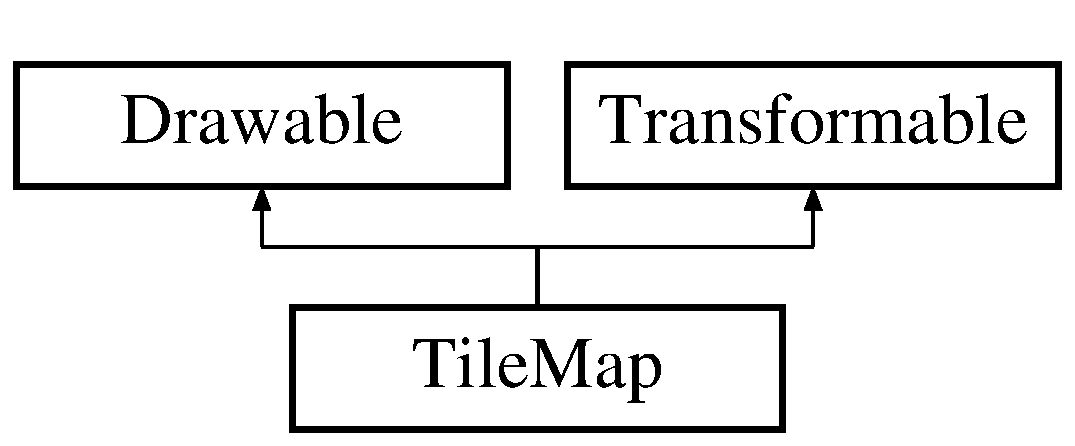
\includegraphics[height=2.000000cm]{class_tile_map}
\end{center}
\end{figure}
\subsection*{Public Member Functions}
\begin{DoxyCompactItemize}
\item 
bool \hyperlink{class_tile_map_a5bc3325e2382599c3f986ac64481e832}{load} (const std\+::string \&tileset, sf\+::\+Vector2u tile\+Size, const int $\ast$tiles, unsigned int width, unsigned int height)
\begin{DoxyCompactList}\small\item\em This attempts to load and populate the Vertex\+Array used for the tilemap. \end{DoxyCompactList}\end{DoxyCompactItemize}


\subsection{Detailed Description}
Consists of a Vertex\+Array of tiles, and a Texture the \hyperlink{class_tile_map}{Tile\+Map} is constructed from. 

\subsection{Member Function Documentation}
\mbox{\Hypertarget{class_tile_map_a5bc3325e2382599c3f986ac64481e832}\label{class_tile_map_a5bc3325e2382599c3f986ac64481e832}} 
\index{Tile\+Map@{Tile\+Map}!load@{load}}
\index{load@{load}!Tile\+Map@{Tile\+Map}}
\subsubsection{\texorpdfstring{load()}{load()}}
{\footnotesize\ttfamily bool Tile\+Map\+::load (\begin{DoxyParamCaption}\item[{const std\+::string \&}]{tileset,  }\item[{sf\+::\+Vector2u}]{tile\+Size,  }\item[{const int $\ast$}]{tiles,  }\item[{unsigned int}]{width,  }\item[{unsigned int}]{height }\end{DoxyParamCaption})}



This attempts to load and populate the Vertex\+Array used for the tilemap. 


\begin{DoxyParams}{Parameters}
{\em tileset} & The name of the texture file to load \\
\hline
{\em tile\+Size} & The size of the requested tile (x, y) \\
\hline
{\em tiles} & An array of integers representing which tile from the tilesheet to load \\
\hline
{\em width} & The number of tiles representing the width of the \hyperlink{class_tile_map}{Tile\+Map} \\
\hline
{\em height} & The number of tiles representing the height of the \hyperlink{class_tile_map}{Tile\+Map} \\
\hline
\end{DoxyParams}
\begin{DoxyReturn}{Returns}
true if the tilemap was loaded correctly, false if it was not 
\end{DoxyReturn}


The documentation for this class was generated from the following files\+:\begin{DoxyCompactItemize}
\item 
Summer\+Workshop2\+D/\hyperlink{_tile_map_8h}{Tile\+Map.\+h}\item 
Summer\+Workshop2\+D/\hyperlink{_tile_map_8cpp}{Tile\+Map.\+cpp}\end{DoxyCompactItemize}

\chapter{File Documentation}
\hypertarget{main_8cpp}{}\section{main.\+cpp File Reference}
\label{main_8cpp}\index{main.\+cpp@{main.\+cpp}}
{\ttfamily \#include $<$S\+F\+M\+L\textbackslash{}graphics.\+hpp$>$}\newline
{\ttfamily \#include $<$stdlib.\+h$>$}\newline
{\ttfamily \#include $<$vector$>$}\newline
{\ttfamily \#include $<$time.\+h$>$}\newline
{\ttfamily \#include \char`\"{}Summer\+Workshop2\+D\textbackslash{}\+Animation.\+h\char`\"{}}\newline
{\ttfamily \#include \char`\"{}Summer\+Workshop2\+D\textbackslash{}\+Collision.\+h\char`\"{}}\newline
{\ttfamily \#include \char`\"{}Summer\+Workshop2\+D\textbackslash{}\+Tile\+Map.\+h\char`\"{}}\newline
\subsection*{Macros}
\begin{DoxyCompactItemize}
\item 
\#define \hyperlink{main_8cpp_af97760b86fa45f374a22be0f2cb5b0fa}{S\+E\+C\+O\+N\+D\+S\+\_\+\+P\+E\+R\+\_\+\+F\+R\+A\+ME}~16
\begin{DoxyCompactList}\small\item\em The number of milliseconds per frame of animation. \end{DoxyCompactList}\end{DoxyCompactItemize}
\subsection*{Functions}
\begin{DoxyCompactItemize}
\item 
void \hyperlink{main_8cpp_a811b7cf72f3317200595c3a353431608}{Input} ()
\begin{DoxyCompactList}\small\item\em This takes input and that\textquotesingle{}s about it. \end{DoxyCompactList}\item 
void \hyperlink{main_8cpp_aec0783b5a136e042adcc47bae4fe5291}{Update} ()
\begin{DoxyCompactList}\small\item\em This updates the world. \end{DoxyCompactList}\item 
void \hyperlink{main_8cpp_a2fc8720d089408eea6ff617be7149b44}{Draw\+Shit} ()
\begin{DoxyCompactList}\small\item\em This draws shit. \end{DoxyCompactList}\item 
int \hyperlink{main_8cpp_a3c04138a5bfe5d72780bb7e82a18e627}{main} (int argc, char $\ast$$\ast$argv)
\begin{DoxyCompactList}\small\item\em The the heart of operations. \end{DoxyCompactList}\end{DoxyCompactItemize}


\subsection{Macro Definition Documentation}
\mbox{\Hypertarget{main_8cpp_af97760b86fa45f374a22be0f2cb5b0fa}\label{main_8cpp_af97760b86fa45f374a22be0f2cb5b0fa}} 
\index{main.\+cpp@{main.\+cpp}!S\+E\+C\+O\+N\+D\+S\+\_\+\+P\+E\+R\+\_\+\+F\+R\+A\+ME@{S\+E\+C\+O\+N\+D\+S\+\_\+\+P\+E\+R\+\_\+\+F\+R\+A\+ME}}
\index{S\+E\+C\+O\+N\+D\+S\+\_\+\+P\+E\+R\+\_\+\+F\+R\+A\+ME@{S\+E\+C\+O\+N\+D\+S\+\_\+\+P\+E\+R\+\_\+\+F\+R\+A\+ME}!main.\+cpp@{main.\+cpp}}
\subsubsection{\texorpdfstring{S\+E\+C\+O\+N\+D\+S\+\_\+\+P\+E\+R\+\_\+\+F\+R\+A\+ME}{SECONDS\_PER\_FRAME}}
{\footnotesize\ttfamily \#define S\+E\+C\+O\+N\+D\+S\+\_\+\+P\+E\+R\+\_\+\+F\+R\+A\+ME~16}



The number of milliseconds per frame of animation. 

\begin{DoxyAuthor}{Author}
Matt Kataryniak 
\end{DoxyAuthor}


\subsection{Function Documentation}
\mbox{\Hypertarget{main_8cpp_a2fc8720d089408eea6ff617be7149b44}\label{main_8cpp_a2fc8720d089408eea6ff617be7149b44}} 
\index{main.\+cpp@{main.\+cpp}!Draw\+Shit@{Draw\+Shit}}
\index{Draw\+Shit@{Draw\+Shit}!main.\+cpp@{main.\+cpp}}
\subsubsection{\texorpdfstring{Draw\+Shit()}{DrawShit()}}
{\footnotesize\ttfamily void Draw\+Shit (\begin{DoxyParamCaption}{ }\end{DoxyParamCaption})}



This draws shit. 

\begin{DoxyReturn}{Returns}
N\+U\+LL 
\end{DoxyReturn}
\mbox{\Hypertarget{main_8cpp_a811b7cf72f3317200595c3a353431608}\label{main_8cpp_a811b7cf72f3317200595c3a353431608}} 
\index{main.\+cpp@{main.\+cpp}!Input@{Input}}
\index{Input@{Input}!main.\+cpp@{main.\+cpp}}
\subsubsection{\texorpdfstring{Input()}{Input()}}
{\footnotesize\ttfamily void Input (\begin{DoxyParamCaption}{ }\end{DoxyParamCaption})}



This takes input and that\textquotesingle{}s about it. 

\begin{DoxyReturn}{Returns}
N\+U\+LL 
\end{DoxyReturn}
\mbox{\Hypertarget{main_8cpp_a3c04138a5bfe5d72780bb7e82a18e627}\label{main_8cpp_a3c04138a5bfe5d72780bb7e82a18e627}} 
\index{main.\+cpp@{main.\+cpp}!main@{main}}
\index{main@{main}!main.\+cpp@{main.\+cpp}}
\subsubsection{\texorpdfstring{main()}{main()}}
{\footnotesize\ttfamily int main (\begin{DoxyParamCaption}\item[{int}]{argc,  }\item[{char $\ast$$\ast$}]{argv }\end{DoxyParamCaption})}



The the heart of operations. 


\begin{DoxyParams}{Parameters}
{\em argc} & Count of arguments \\
\hline
{\em argv} & Array of character arguments \\
\hline
\end{DoxyParams}
\begin{DoxyReturn}{Returns}
0 if good, 1 if error 
\end{DoxyReturn}
\mbox{\Hypertarget{main_8cpp_aec0783b5a136e042adcc47bae4fe5291}\label{main_8cpp_aec0783b5a136e042adcc47bae4fe5291}} 
\index{main.\+cpp@{main.\+cpp}!Update@{Update}}
\index{Update@{Update}!main.\+cpp@{main.\+cpp}}
\subsubsection{\texorpdfstring{Update()}{Update()}}
{\footnotesize\ttfamily void Update (\begin{DoxyParamCaption}{ }\end{DoxyParamCaption})}



This updates the world. 

\begin{DoxyReturn}{Returns}
N\+U\+LL 
\end{DoxyReturn}

\hypertarget{_animation_8h}{}\section{Summer\+Workshop2\+D/\+Animation.h File Reference}
\label{_animation_8h}\index{Summer\+Workshop2\+D/\+Animation.\+h@{Summer\+Workshop2\+D/\+Animation.\+h}}
{\ttfamily \#include $<$S\+F\+M\+L\textbackslash{}graphics.\+hpp$>$}\newline
\subsection*{Classes}
\begin{DoxyCompactItemize}
\item 
struct \hyperlink{struct_animation}{Animation}
\begin{DoxyCompactList}\small\item\em This is an animation structure. \end{DoxyCompactList}\end{DoxyCompactItemize}
\subsection*{Macros}
\begin{DoxyCompactItemize}
\item 
\#define \hyperlink{_animation_8h_aefcfbff62033a5293157520b346713fb}{M\+A\+X\+\_\+\+F\+R\+A\+M\+E\+S\+\_\+\+P\+E\+R\+\_\+\+A\+N\+I\+M\+A\+T\+I\+ON}~11
\begin{DoxyCompactList}\small\item\em The maximum number of frames a single animation can have. \end{DoxyCompactList}\end{DoxyCompactItemize}


\subsection{Macro Definition Documentation}
\mbox{\Hypertarget{_animation_8h_aefcfbff62033a5293157520b346713fb}\label{_animation_8h_aefcfbff62033a5293157520b346713fb}} 
\index{Animation.\+h@{Animation.\+h}!M\+A\+X\+\_\+\+F\+R\+A\+M\+E\+S\+\_\+\+P\+E\+R\+\_\+\+A\+N\+I\+M\+A\+T\+I\+ON@{M\+A\+X\+\_\+\+F\+R\+A\+M\+E\+S\+\_\+\+P\+E\+R\+\_\+\+A\+N\+I\+M\+A\+T\+I\+ON}}
\index{M\+A\+X\+\_\+\+F\+R\+A\+M\+E\+S\+\_\+\+P\+E\+R\+\_\+\+A\+N\+I\+M\+A\+T\+I\+ON@{M\+A\+X\+\_\+\+F\+R\+A\+M\+E\+S\+\_\+\+P\+E\+R\+\_\+\+A\+N\+I\+M\+A\+T\+I\+ON}!Animation.\+h@{Animation.\+h}}
\subsubsection{\texorpdfstring{M\+A\+X\+\_\+\+F\+R\+A\+M\+E\+S\+\_\+\+P\+E\+R\+\_\+\+A\+N\+I\+M\+A\+T\+I\+ON}{MAX\_FRAMES\_PER\_ANIMATION}}
{\footnotesize\ttfamily \#define M\+A\+X\+\_\+\+F\+R\+A\+M\+E\+S\+\_\+\+P\+E\+R\+\_\+\+A\+N\+I\+M\+A\+T\+I\+ON~11}



The maximum number of frames a single animation can have. 


\hypertarget{_collision_8cpp}{}\section{Summer\+Workshop2\+D/\+Collision.cpp File Reference}
\label{_collision_8cpp}\index{Summer\+Workshop2\+D/\+Collision.\+cpp@{Summer\+Workshop2\+D/\+Collision.\+cpp}}
{\ttfamily \#include $<$S\+F\+M\+L\textbackslash{}graphics.\+hpp$>$}\newline

\hypertarget{_collision_8h}{}\section{Summer\+Workshop2\+D/\+Collision.h File Reference}
\label{_collision_8h}\index{Summer\+Workshop2\+D/\+Collision.\+h@{Summer\+Workshop2\+D/\+Collision.\+h}}
{\ttfamily \#include $<$S\+F\+M\+L\textbackslash{}graphics.\+hpp$>$}\newline
\subsection*{Functions}
\begin{DoxyCompactItemize}
\item 
int \hyperlink{_collision_8h_aeece29bc461fb24dde217b2b137c863f}{Point\+In\+A\+A\+BB} (sf\+::\+Vector2f t, sf\+::\+Float\+Rect A)
\begin{DoxyCompactList}\small\item\em Takes a Vector2f point and checks to see if it is inside of the Float\+Rect. \end{DoxyCompactList}\item 
int \hyperlink{_collision_8h_af446aa23609297d29b78d07c5f4c213f}{A\+A\+B\+Bin\+A\+A\+BB} (sf\+::\+Float\+Rect A, sf\+::\+Float\+Rect B)
\begin{DoxyCompactList}\small\item\em Checks to see if two Float\+Rects have collided with each other. \end{DoxyCompactList}\end{DoxyCompactItemize}


\subsection{Function Documentation}
\mbox{\Hypertarget{_collision_8h_af446aa23609297d29b78d07c5f4c213f}\label{_collision_8h_af446aa23609297d29b78d07c5f4c213f}} 
\index{Collision.\+h@{Collision.\+h}!A\+A\+B\+Bin\+A\+A\+BB@{A\+A\+B\+Bin\+A\+A\+BB}}
\index{A\+A\+B\+Bin\+A\+A\+BB@{A\+A\+B\+Bin\+A\+A\+BB}!Collision.\+h@{Collision.\+h}}
\subsubsection{\texorpdfstring{A\+A\+B\+Bin\+A\+A\+B\+B()}{AABBinAABB()}}
{\footnotesize\ttfamily int A\+A\+B\+Bin\+A\+A\+BB (\begin{DoxyParamCaption}\item[{sf\+::\+Float\+Rect}]{A,  }\item[{sf\+::\+Float\+Rect}]{B }\end{DoxyParamCaption})}



Checks to see if two Float\+Rects have collided with each other. 


\begin{DoxyParams}{Parameters}
{\em A} & The first Float\+Rect \\
\hline
{\em B} & The second Float\+Rect \\
\hline
\end{DoxyParams}
\begin{DoxyReturn}{Returns}
1 if Float\+Rects are colliding, 0 if they are not 
\end{DoxyReturn}
\mbox{\Hypertarget{_collision_8h_aeece29bc461fb24dde217b2b137c863f}\label{_collision_8h_aeece29bc461fb24dde217b2b137c863f}} 
\index{Collision.\+h@{Collision.\+h}!Point\+In\+A\+A\+BB@{Point\+In\+A\+A\+BB}}
\index{Point\+In\+A\+A\+BB@{Point\+In\+A\+A\+BB}!Collision.\+h@{Collision.\+h}}
\subsubsection{\texorpdfstring{Point\+In\+A\+A\+B\+B()}{PointInAABB()}}
{\footnotesize\ttfamily int Point\+In\+A\+A\+BB (\begin{DoxyParamCaption}\item[{sf\+::\+Vector2f}]{t,  }\item[{sf\+::\+Float\+Rect}]{A }\end{DoxyParamCaption})}



Takes a Vector2f point and checks to see if it is inside of the Float\+Rect. 


\begin{DoxyParams}{Parameters}
{\em t} & The point to test \\
\hline
{\em A} & The Float\+Rect to test \\
\hline
\end{DoxyParams}
\begin{DoxyReturn}{Returns}
1 if point is inside Float\+Rect, 0 if the point is not 
\end{DoxyReturn}

\hypertarget{_tile_map_8cpp}{}\section{Summer\+Workshop2\+D/\+Tile\+Map.cpp File Reference}
\label{_tile_map_8cpp}\index{Summer\+Workshop2\+D/\+Tile\+Map.\+cpp@{Summer\+Workshop2\+D/\+Tile\+Map.\+cpp}}
{\ttfamily \#include $<$S\+F\+M\+L\textbackslash{}graphics.\+hpp$>$}\newline
{\ttfamily \#include \char`\"{}Tile\+Map.\+h\char`\"{}}\newline

\hypertarget{_tile_map_8h}{}\section{Summer\+Workshop2\+D/\+Tile\+Map.h File Reference}
\label{_tile_map_8h}\index{Summer\+Workshop2\+D/\+Tile\+Map.\+h@{Summer\+Workshop2\+D/\+Tile\+Map.\+h}}
{\ttfamily \#include $<$S\+F\+M\+L\textbackslash{}graphics.\+hpp$>$}\newline
\subsection*{Classes}
\begin{DoxyCompactItemize}
\item 
class \hyperlink{class_tile_map}{Tile\+Map}
\begin{DoxyCompactList}\small\item\em Consists of a Vertex\+Array of tiles, and a Texture the \hyperlink{class_tile_map}{Tile\+Map} is constructed from. \end{DoxyCompactList}\end{DoxyCompactItemize}

%--- End generated contents ---

% Index
\backmatter
\newpage
\phantomsection
\clearemptydoublepage
\addcontentsline{toc}{chapter}{Index}
\printindex

\end{document}
